\documentclass{tufte-handout}

% $ W^{(1)} \in \mathbb{R}^{d \times 2d}$

% \left[ \begin{array}{c} h^{(1)}_{Left} \\ h^{(1)}_{Right} \end{array} \right]

%test


\title{CS224n: Deep Learning for NLP\thanks{Course Instructor: Richard Socher} \\
       \Large Lecture Notes: Part VII \thanks{Authors: Francois Chaubard, Richard Socher}}

\date{Winter 2017} % without \date command, current date is supplied

%\geometry{showframe} % display margins for debugging page layout

\usepackage{graphicx} % allow embedded images
\setkeys{Gin}{width=\linewidth,totalheight=\textheight,keepaspectratio}
\graphicspath{{notes7/fig/}} % set of paths to search for images
\usepackage{amsmath}  % extended mathematics
\usepackage{amstext}  % extended text
\usepackage{booktabs} % book-quality tables
\usepackage{units}    % non-stacked fractions and better unit spacing
\usepackage{multicol} % multiple column layout facilities
\usepackage{lipsum}   % filler text
\usepackage{fancyvrb} % extended verbatim environments
\usepackage{placeins}
\usepackage{mdframed}% http://ctan.org/pkg/mdframed
\fvset{fontsize=\normalsize}% default font size for fancy-verbatim environments

% Standardize command font styles and environments
\newcommand{\doccmd}[1]{\texttt{\textbackslash#1}}% command name -- adds backslash automatically
\newcommand{\docopt}[1]{\ensuremath{\langle}\textrm{\textit{#1}}\ensuremath{\rangle}}% optional command argument
\newcommand{\docarg}[1]{\textrm{\textit{#1}}}% (required) command argument
\newcommand{\docenv}[1]{\textsf{#1}}% environment name
\newcommand{\docpkg}[1]{\texttt{#1}}% package name
\newcommand{\doccls}[1]{\texttt{#1}}% document class name
\newcommand{\docclsopt}[1]{\texttt{#1}}% document class option name
\newenvironment{docspec}{\begin{quote}\noindent}{\end{quote}}% command specification environment
\newcommand{\argmin}{\operatornamewithlimits{argmin}}
\newcommand{\argmax}{\operatornamewithlimits{argmax}}
\newcommand{\norm}[1]{\left\lVert#1\right\rVert}
\newcommand{\textunderscript}[1]{$_{\text{#1}}$}
\allowdisplaybreaks
\setcounter{secnumdepth}{3}

\newmdtheoremenv[outerlinewidth=2,leftmargin=40,rightmargin=40,%
    backgroundcolor=lightgray,outerlinecolor=blue,innertopmargin=10pt,%
    splittopskip=\topskip,skipbelow=\baselineskip,%
    skipabove=\baselineskip,ntheorem,roundcorner=5pt]{theorem}{Snippet}[section]

\begin{document}

\maketitle% this prints the handout title, author, and date

%\printclassoptions


\textbf{Keyphrases: RNN, Recursive Neural Networks, MV-RNN, RNTN}

This set of notes discusses and describes the many variants on the RNN (Recursive Neural Networks) and their application and successes in the field of NLP.

\section{Recursive Neural Networks}\label{sec:rnns}

\begin{marginfigure}%
  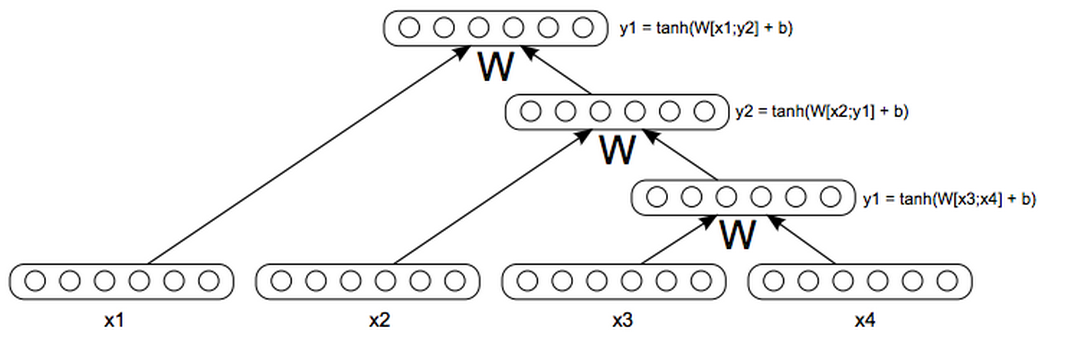
\includegraphics[width=\linewidth]{img1}
  \caption{A standard Recursive Neural Network }
  \label{fig:img1}
\end{marginfigure}

In these notes, we introduce and discuss a new type of model that is indeed a superset of the previously discussed Recurrent Neural Network. Recursive Neural Networks (RNNs) are perfect for settings that have nested hierarchy and an intrinsic recursive structure. Well if we think about a sentence, doesn't this have such a structure? Take the sentence ''A small crowd quietly enters the historical church''. First, we break apart the sentence into its respective Noun Phrase, Verb Phrase, ''A small crowd'' and ''quietly enters the historical church'', respectively. But there is a noun phrase, verb phrase within that verb phrase right? ''quietly enters'' and ''historical church''. etc, etc. Seems pretty recursive to me.

The syntactic rules of language are highly recursive. So we take advantage of that recursive structure with a model that respects it! Another added benefit of modeling sentences with RNN's is that we can now input sentences of arbitrary length, which was a huge head scratcher for using Neural Nets in NLP, with very clever tricks to make the input vector of the sentence to be of equal size despite the length of the sentences not being equal. (see Bengio et al., 2003; Henderson, 2003; Collobert \& Weston, 2008)



\begin{marginfigure}%
  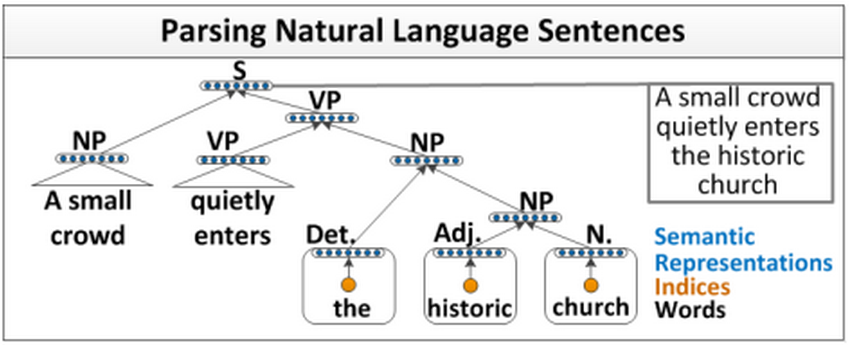
\includegraphics[width=\linewidth]{img2}
  \caption{Parse Tree of a sentence. }
  \label{fig:img2}
\end{marginfigure}

Let's imagine our task is to take a sentence and represent it as a vector in the same semantic space as the words themselves. So that phrases like ''I went to the mall yesterday'', ''We went shopping last week'', and ''They went to the store'', would all be pretty close in distance to each other. Well we have seen ways to train unigram word vectors, should we do the same for bigrams, trigrams, etc. This very well may work but there are two major issues with this thinking. 1) There are literally an infinite amount of possible combinations of words. Storing and training an infinite amount of vectors would just be absurd. 2) Some combinations of words while they might be completely reasonable to hear in language, may never be represented in our training/dev corpus. So we would never learn them.

We need a way to take a sentence and its respective words vectors, and derive what the embedded vector should be. Now lets first ask a very debated question. Is it naive to believe that the vector space that we used to represent all words, is sufficiently expressive to also be able to represent all sentences of any length? While this may be unintuitive, the performance of these models suggest that this is actually a reasonable thing to do.

Let's first discuss the difference between semantic and grammatical understanding of a sentence. Semantic analysis is an understanding of the meaning of a sentence, being able to represent the phrase as a vector in a structured semantic space, where similar sentences are very nearby, and unrelated sentences are very far away. The grammatical understanding is one where we have identified the underlying grammatical structure of the sentence, which part of the sentence depends on which other part, what words are modifying what other words, etc. The output of such an understanding is usually represented as a parse tree as displayed in Figure 2.

Now for the million dollar question. If we want to know the semantic representation, is it an advantage, nay, required, to have a grammatical understanding? Well some might disagree but for now we will treat this semantic composition task the following way. First, we need to understand words. Then, we need to know the way words are put together, Then, finally, we can get to a meaning of a phrase or sentence by leveraging these two previous concepts.

So lets begin with our first model built on this principle. Let's imagine we were given a sentence, and we knew the parse tree for that sentence, such as the one displayed in Figure 2, could we figure out an encoding for the sentence and also perhaps a sentiment score just from the word vectors that are in the sentence? We observe how a Simple RNN can perform this task.
%(As will you in PSet 3!)

\subsection{A simple single layer RNN}


\begin{marginfigure}%
  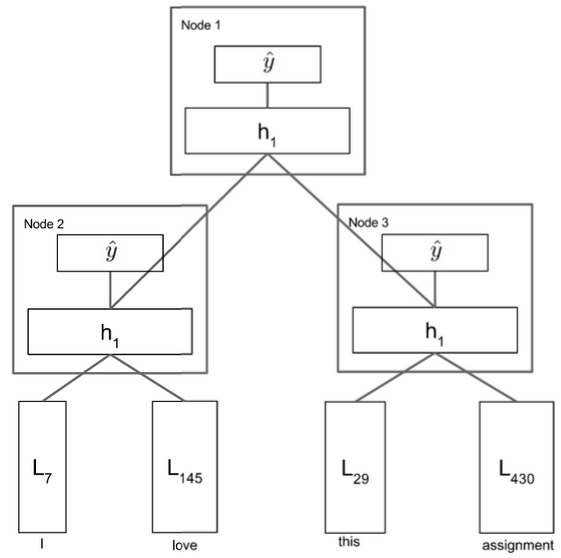
\includegraphics[width=\linewidth]{img3}
  \caption{An example standard RNN applied to a parsed sentence ''I love this assignment'' }
  \label{fig:img3}
\end{marginfigure}

Lets walk through the model displayed in Figure 3 above. We first take a sentence parse tree and the sentence word vectors and begin to walk up the tree. The lowest node in the graph is Node 3, so we concatenate $L_{29}$ and $L_{430}$ to form a vector $\in \mathbb{R}^{2d}$ and feed it into our network to compute:
\begin{equation}
h^{(1)} = tanh(W^{(1)} \left[ \begin{array}{c} L_{29} \\ L_{430} \end{array} \right] + b^{(1)})
\end{equation}
Since $ W^{(1)} \in \mathbb{R}^{d \times 2d}$ and $ b^{(1)} \in \mathbb{R}^{d}$, $ h^{(1)} \in \mathbb{R}^{d}$. We can now think of $h^{(1)}$ as a point in the same word vector space for the bigram ''this assignment'', in which we did not need to learn this representation separately, but rather derived it from its constituting word vectors.

We now take $h^{(1)}$ and put it through a softmax layer to get a score over a set of sentiment classes, a discrete set of known classes that represent some meaning. In the case of positive/negative sentiment analysis, we would have 5 classes, class 0 implies strongly negative, class 1 implies negative, class 2 is neutral, class 3 is positive, and finally class 4 is strongly positive.

Now we do the same thing with the ''I'' and ''love'' to produce the vector $h^{(1)}$ for the phrase ''I love''. Again, we compute a score over the semantic classes again for that phrase. Finally, for the most interesting step, we need to merge the two phrases ''I love'' and ''this assignment''. Here we are concatenating word phrases, rather than word vectors! We do this in the same manner, concatenating the two $h^{(1)}$ vectors and compute
\begin{equation}
 h^{(1)} = \text{tanh}(W^{(1)}  \left[ \begin{array}{c} h^{(1)}_{Left} \\ h^{(1)}_{Right} \end{array} \right] + b^{(1)})
\end{equation}

Now we have a vector in the word vector space that represents the full sentence ''I love this assignment''. Furthermore, we can put this $h^{(1)}$ through the same softmax layer as before, and compute sentiment probabilities for the full sentence. Of course the model will only do this reliably once trained.
%but that left for you to do in PSet3. :)

Now lets take a step back. First, is it naive to think we can use the same matrix W to concatenate all words together and get a very expressive $h^{(1)}$ and yet again use that same matrix W to concatenate all phrase vectors to get even deeper phrases? These criticisms are valid and we can address them in the following twist on the simple RNN.

\subsection{Syntactically Untied SU-RNN}


\begin{marginfigure}%
  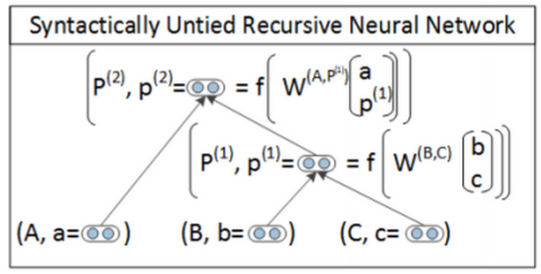
\includegraphics[width=\linewidth]{img4}
  \caption{Using different W's for different categories of inputs is more natural than having just one W for all categories }
  \label{fig:img4}
\end{marginfigure}

As we discussed in the criticisms of the previous section, using the same W to bring together a Noun Phrase and Verb Phrase and to bring together a Prepositional Phrase and another word vector seems intuitively wrong. And maybe we are bluntly merging all of these functionalities into too weak of a model.

What we can do to remedy this shortcoming is to ''syntactically untie'' the weights of these different tasks. By this we mean, there is no reason to expect the optimal W for one category of inputs to be at all related to the optimal W for another category of inputs. So we let these W's be different and relax this constraint. While this for sure increases our weight matrices to learn, the performance boost we gain is non-trivial.

As in FIgure 4 above, we notice our model is now conditioned upon what the syntactic categories of the inputs are. Note, we determine what the categories are via a very simple Probabilistic Context Free Grammar (PCFG) which is more or less learned by computing summary statistics over the Penn Tree Bank to learn rules such as ''The'' is always a DT, etc, etc. No deeper understanding of this part is really necessary, just know it\'s really simple.

The only major other difference in this model is that we initialize the W's to the identity. This way the default thing to do is to average the two word vectors coming in. Slowly but surely, the model learns which vector is more important and also any rotation or scaling of the vectors that improve performance. We observe in Figure 5 that the trained weight matrices learn actually meaning!  For example, the DT-NP rule or Determiner followed by a Noun Phrase such as ''The cat'' or ''A man'', puts more emphasis on the Noun Phrase than on the Determiner. (this is obvious because the right diagonals are red meaning higher weightl). This is called the notion of soft head words, which is something that Linguists have long observed to be true for sometime, however the model learned this on its own just by looking at data. Pretty cool!

\begin{marginfigure}%
  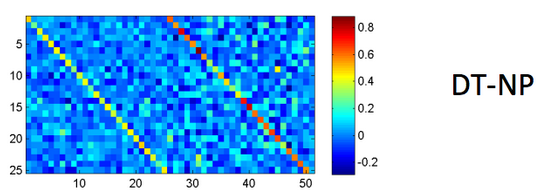
\includegraphics[width=\linewidth]{img5}
  \caption{The learnt W weights for DT-NP composition match Linguists theory }
  \label{fig:img5}
\end{marginfigure}

The SU-RNN does indeed outperform previously discussed models but perhaps it is still not expressive enough. If we think of modifying words, such as adverbs like ''very'', any interpolation with this word vector and the following one, is definitely not what the understood nature of ''very'' is.

As an adverb, it's literal definition is ''used for emphasis''. How can we have a vector that emphasizes any other vector that is to follow when we are solely performing a linear interpolation? How can we construct a vector that will ''scale'' any other vector this way? Truth is we can not. We need to have some form of multiplication of word on another word. We uncover two such compositions below that enable this. The first utilizes word matrices and the other utilizes a Quadratic equation over the typical Affine.


\subsection{MV-RNN's (Matrix-Vector Recursive Neural Networks)}


\begin{marginfigure}%
  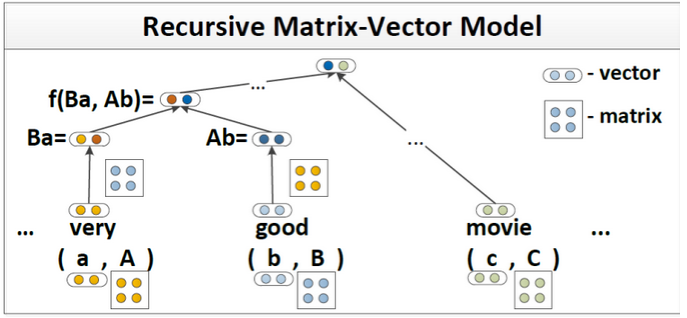
\includegraphics[width=\linewidth]{img6}
  \caption{An example MV-RNN}
  \label{fig:img6}
\end{marginfigure}

We now augment our word representation, to not only include a word vector, but also a word matrix! So the word ''very'' will have a word vector  $v_{very} \in \mathbb{R}^{d}$ but also $V_{very} \in \mathbb{R}^{d\times d}$. This gives us the expressive ability to not only embed what a word means, but we also learn the way that words ''modify'' other words. The word matrix enables the latter. To feed two words, $a$ and $b$, into a RNN, we take their word matrices $A$ and $B$, to form our input vector x as the concatenation of vector $Ab$ and $Ba$. For our example of ''very'', $V_{very}$ could just be the identity times any scalar above one. Which would scale any neighboring word vector by that number! This is the type of expressive ability we desired. While the new word representation explodes our feature space, we can express much better the way words modify each other.

By observing the errors the model makes, we see even the MV-RNN still can not express certain relations. We observe three major classes of mistakes.

First, Negated Positives. When we say something positive but one word turns it negative, the model can not weigh that one word strong enough to flip the sentiment of the entire sentence. Figure 7 shows such an example where the swap of the word ''most'' to ''least'' should flip the entire sentiment of the sentence, but the MV-RNN does not capture this successfully.



\begin{marginfigure}%
  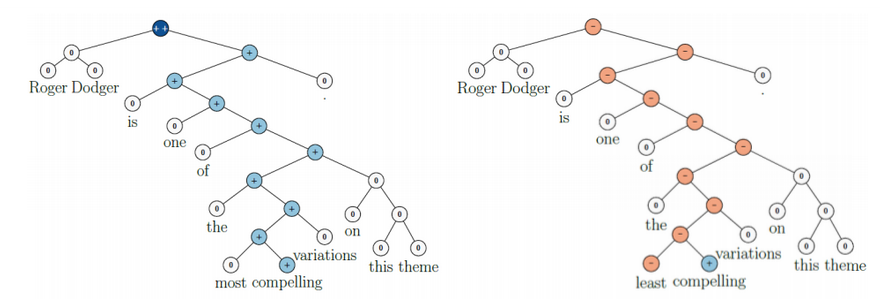
\includegraphics[width=\linewidth]{img7}
  \caption{Negated Positives}
  \label{fig:img7}
\end{marginfigure}

The second class of mistakes is the Negated Negative case. Where we say something is not bad, or not dull, as in Figure 8. The MV-RNN can not recognize that the word ''not'' lessens the sentiment from negative to neutral.


\begin{marginfigure}%
  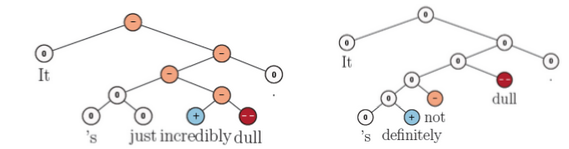
\includegraphics[width=\linewidth]{img8}
  \caption{Negated Negatives}
  \label{fig:img8}
\end{marginfigure}

The final class of errors we observe is the ''X but Y conjunction'' displayed in Figure 9. Here the X might be negative BUT if the Y is positive then the model's sentiment output for the sentence should be positive! MV-RNNs struggle with this.

\begin{marginfigure}%
  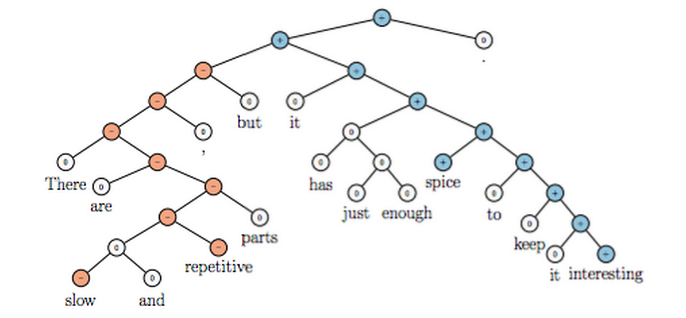
\includegraphics[width=\linewidth]{img9}
  \caption{Using a Recursive Neural Net can correctly classify the sentiment of the contrastive conjunction X but Y but the MV-RNN can not}
  \label{fig:img9}
\end{marginfigure}

Thus, we must look for an even more expressive composition algorithm that will be able to fully capture these types of high level compositions.

\subsection{RNTNs (Recursive Neural Tensor Network)}

The final RNN we will cover here is by far the most successful on the three types of errors we left off with. The Recursive Neural Tensor Network does away with the notion of a word matrix, and furthermore, does away with the traditional affine transformation pre-tanh/sigmoid concept. To compose two word vectors or phrase vectors, we again concatenate them to form a vector $\in \mathbb{R}^{2d}$ but instead of putting it through an affine function then a nonlinear, we put it through a quadratic first, then a nonlinear, such as:
\begin{equation}
h^{(1)} = tanh(x^T V x + Wx)
\end{equation}

Note that $V$ is a 3rd order tensor in $\in \mathbb{R}^{2d \times 2d \times d}$.  We compute $ x^T V[i] x $  $\forall i \in [1, 2, ... d]$ slices of the tensor outputting a vector $\in \mathbb{R}^{d}$. We then add $Wx$ and put it through a nonlinear function. The quadratic shows that we can indeed allow for the multiplicative type of interaction between the word vectors without needing to maintain and learn word matrices!


\begin{marginfigure}%
  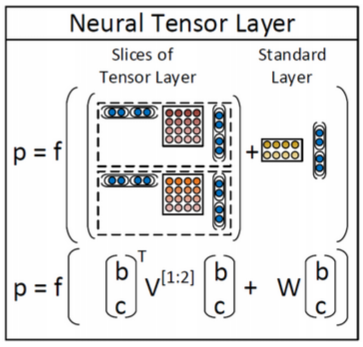
\includegraphics[width=\linewidth]{img10}
  \caption{One slice of a RNTN. Note there would be d of these slices.}
  \label{fig:img10}
\end{marginfigure}


\begin{marginfigure}%
  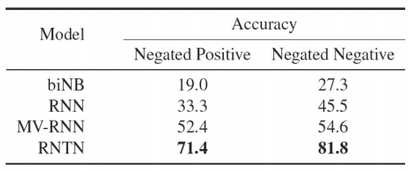
\includegraphics[width=\linewidth]{img11}
  \caption{Comparing performance on the Negated Positive and Negated Negative data sets.}
  \label{fig:img11}
\end{marginfigure}

As we see in Figure 11, the RNTN is the only model that is capable of succeeding on these very hard datasets.

We will continue next time with a model that actually outperforms the RNTN in some aspects and it does not require an input parse tree! This model is the Dynamic Convolutional Neural Network, and we will talk about that soon.
%Good luck on your midterm!

\section{CNNs (Convolutional Neural Networks)}
Back to sentence representation, what if you did NOT know the parse tree? The RecNNs we have observed in this set of lecture notes depend on such an initial parsing. What if we are using Recurrent Networks and the context of the phrase is on its right side? If we only applied Softmax on the last time-step, then the last few words would have a disproportionately large impact on the output, e.g.Sentiment Classification.

\subsection{Why CNNs?}
Convolutional Neural Networks take in a sentence of word vectors and first create a phrase vector for all subphrases, not just grammatically correct phrases (as with Recursive Neural Network)! And then, CNNs group them together for the task at hand.

\subsection{What is Convolution?}
Let's start with the 1D case. Consider two 1D vectors, $f$ and $g$ with $f$ being our primary vector and $g$ corresponding to the filter. The convolution between $f$ and $g$, evaluated at entry $n$ is represented as $(f*g)[n]$ and is equal to $\sum\limits_{m=-M}^Mf[n-m]g[m]$. \\
Figure \ref{fig:2d_conv} shows the 2D convolution case. The $9\times 9$ green matrix represents the primary matrix of concern, $f$. The $3\times 3$ matrix of red numbers represents the filter $g$ and the convolution currently being evaluated is at position $[2,2]$. Figure \ref{fig:2d_conv} shows the value of the convolution at position $[2,2]$ as 4 in the second table. Can you complete the second table?

\begin{marginfigure}%
  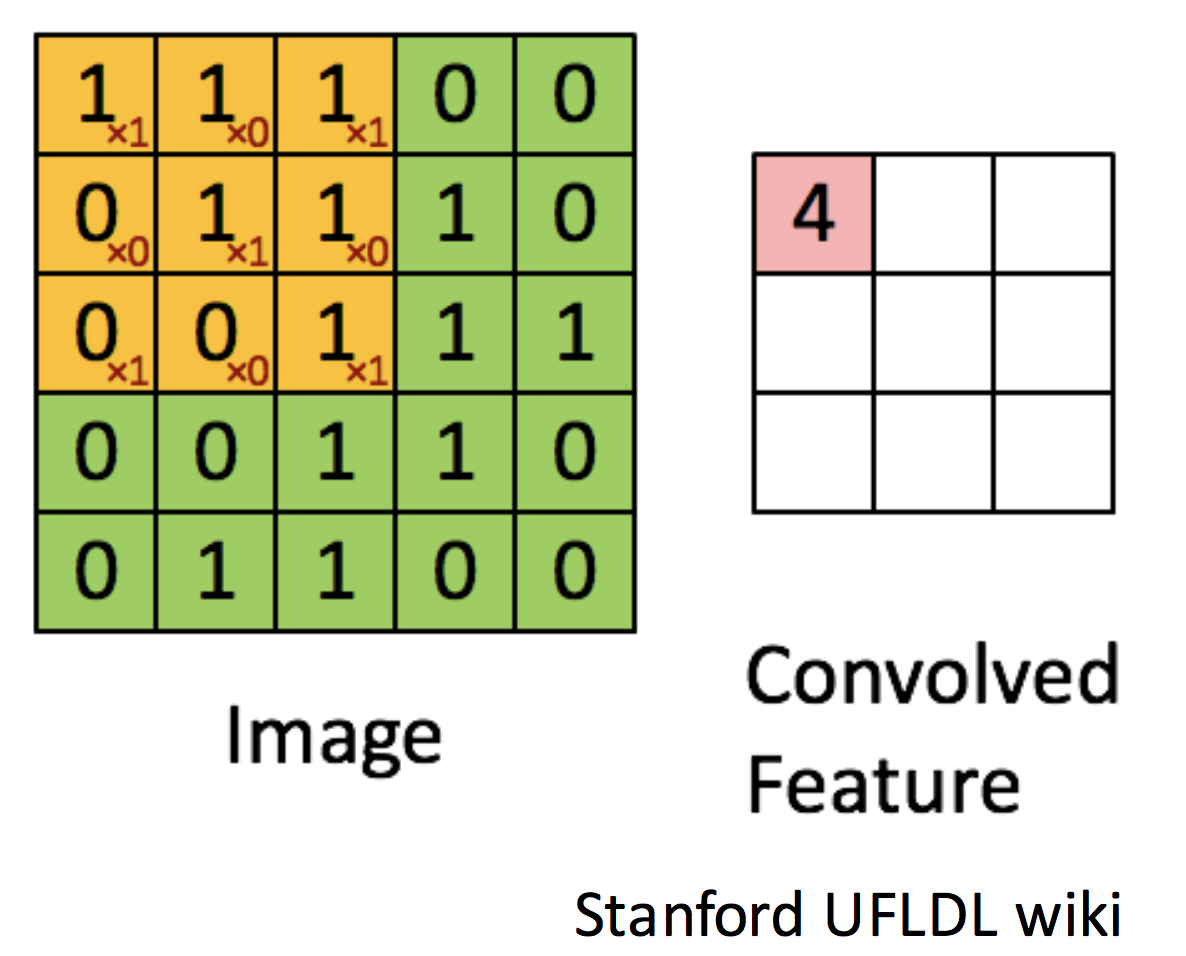
\includegraphics[width=\linewidth]{2d_convolution}
  \caption{Convolution in the 2D case}
  \label{fig:2d_conv}
\end{marginfigure}

\subsection{A Single-Layer CNN}
Consider word-vectors $x_i\in R^k$ and the concatenated word-vectors of a n-word sentence, $x_{1:n}=x_1\oplus x_2...\oplus x_n$. Finally, consider a Convolutional filter $w\in R^{hk}$ i.e. over $h$ words. For $k=2$, $n=5$ and $h=3$, Figure \ref{fig:single_conv} shows the  Single-Layer Convolutional layer for NLP. We will get a single value for each possible combination of three consecutive words in the sentence, "the country of my birth". Note, the filter $w$ is itself a vector and we will have $c_i=f(w^Tx_{i:i|h-1}+b)$ to give $\textbf{c}=[c_1,c_2... c_{n-h+1}]\in R^{n-h+1}$. For the last two time-steps, i.e. starting with the words "my" or "birth", we don't have enough word-vectors to multiply with the  filter (since $h=3$). If we necessarily need the convolutions associated with the last two word-vectors, a common trick is to pad the sentence with $h-1$ zero-vectors at its right-hand-side as in Figure \ref{fig:single_conv_complete}.

\begin{marginfigure}%
  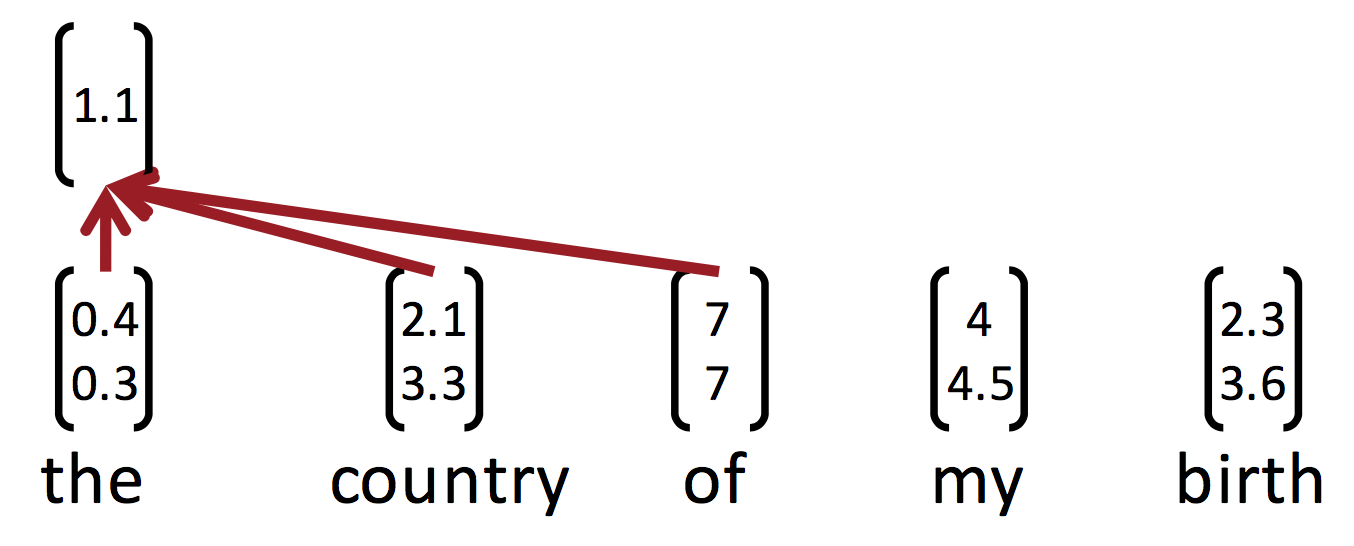
\includegraphics[width=\linewidth]{single-conv}
  \caption{Single-Layer Convolution: one-step}
  \label{fig:single_conv}
\end{marginfigure}

\begin{marginfigure}%
  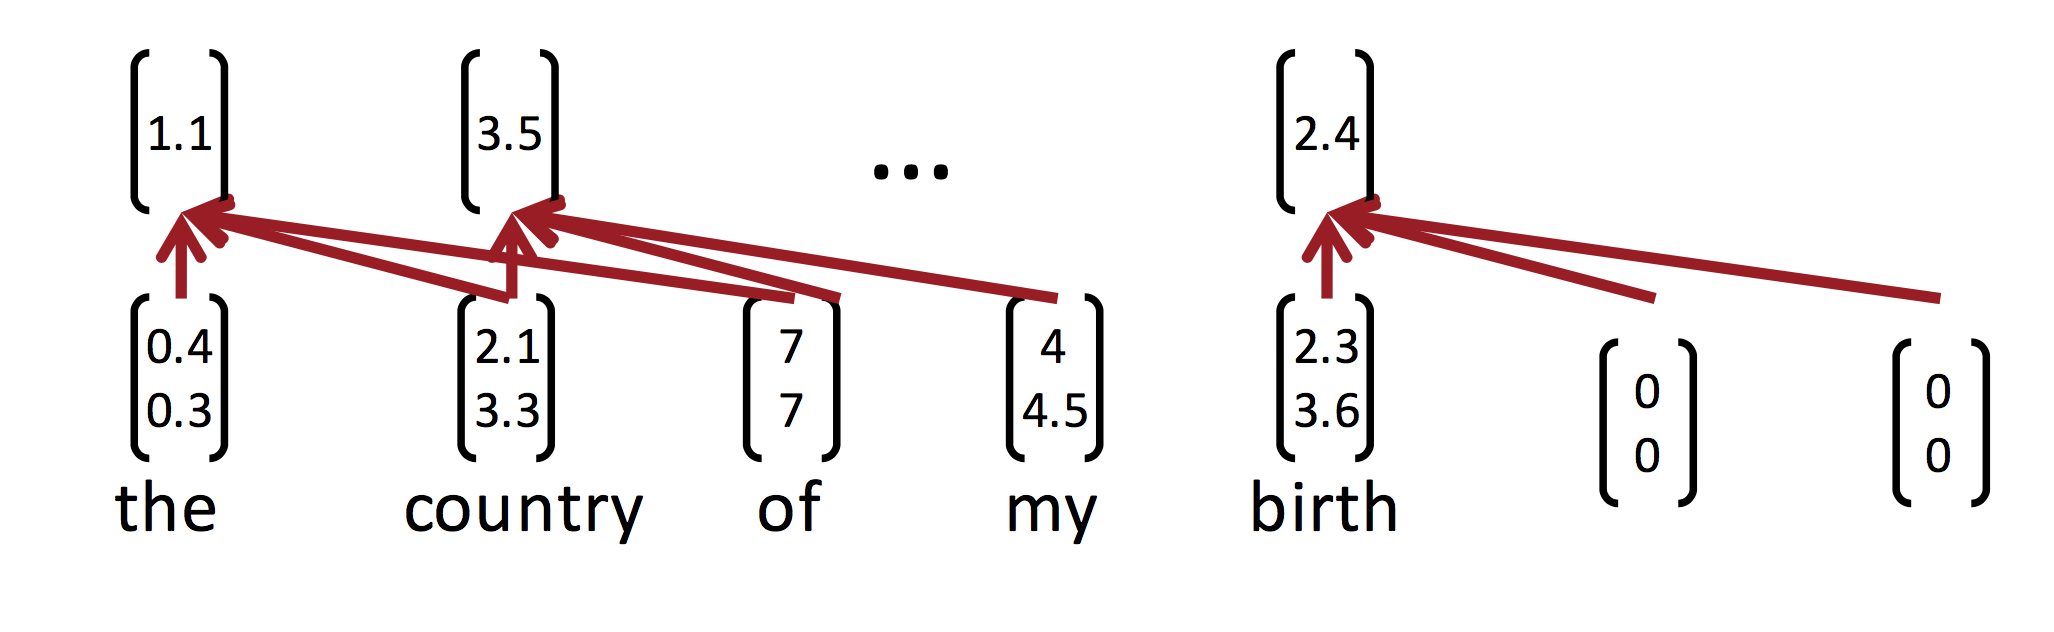
\includegraphics[width=\linewidth]{single-conv-complete}
  \caption{Single-Layer Convolution: all-steps}
  \label{fig:single_conv_complete}
\end{marginfigure}

\subsection{Pooling}
Assuming that we don't use zero-padding, we will get a final convolutional output, $\textbf{c}$ which has $n-h+1$ numbers. Typically, we want to take the outputs of the CNN and feed it as input to further layers like a Feedforward Neural Network or a RecNN. But, all of those need a fixed length input while our CNN output has a length dependent on the length of the sentence, $n$. One clever way to fix this problem is to use max-pooling. The output of the CNN, $\textbf{c}\in \mathbb{R}^{n-h-1}$ is the input to the max-pooling layer. The output of the max-pooling layer is $\hat{c}=max\{\textbf{c}\}$, thus $\hat{c}\in \mathbb{R}$. \\
We could also have used min-pooling because typically we use ReLU as our non-linear activation function and ReLU is bounded on the  low side to 0. Hence a min-pool layer might get smothered by ReLU, so we nearly always use max-pooling over min-pooling.

\subsection{Multiple-Filters}
In the example above related to Figure \ref{fig:single_conv}, we had $h=2$, meaning we looked only at bi-gram with a single specific combination method i.e. filter. We can use multiple bi-gram filters because each filter will learn to recognize a different kind of bi-gram. Even more generally, we are not restricted to using just bi-grams, we can also have filters using tri-grams, quad-grams and even higher lengths. Each filter has an associated max-pool layer. Thus, our final output from the CNN layers will be a vector having length equal to the number of filters.

\subsection{Multiple-Channels}
If we allow gradients to flow into the word-vectors being used here, then the word-vectors might change significantly over training. This is desirable, as it specializes the word-vectors to the specific task at hand (away from say GloVe initialization). But, what about  words that appear only in the test set but not in the train set? While other semantically related word vectors which appear in the train set will have moved significantly from their starting point, such words will still be at their initialization point. The neural network will be specialized for inputs which have been updated. Hence, we will get low performance on sentences with such words (words that are in test but not in train). \\
One work-around is to maintain two sets of word-vectors, one 'static' (no gradient flow into them) and one 'dynamic', which are updated via SGD. Both are initially the same (GloVe or other initialization). Both sets are simultaneously used as input to the neural network. Thus, the initialized word-vectors will always play a role in the training of the neural network. Giving unseen words present in the test set a better chance of being interpreted  correctly. \\
There are several ways of handling these two channels, most common is to simply average them before using in a CNN. The other method is to double the length of the CNN filters.

\subsection{CNN Options}
\begin{enumerate}
\item  Narrow vs Wide \\
Refer to Figure \ref{fig:narrow_vs_wide}. Another way to ask this is  should we not (narrow) or should we (wide) zero-pad? If we use Narrow Convolution, we compute a convolution only in those positions where all the components of a filter have a matching input component. This will clearly not be the case at the start and end boundaries of the input, as in the left side network in Figure \ref{fig:narrow_vs_wide}. If we use Wide Convolution, we have an output component corresponding to each alignment of the convolution filter. For this, we will have to pad the input at the start and the end with $h-1$ zeros. \\
In the Narrow Convolution case, the output length will be $n-h+1$ and in the Wide Convolution case, the length will be $n+h-1$.

\begin{marginfigure}%
  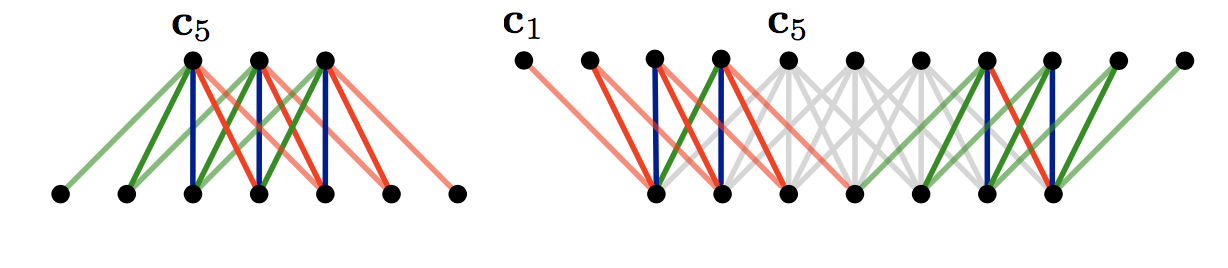
\includegraphics[width=\linewidth]{narrow_vs_wide}
  \caption{Narrow and Wide Convolution (from Kalchbrenner et al. (2014))}
  \label{fig:narrow_vs_wide}
\end{marginfigure}

\item  $k$-max pooling\\
This is a generalization of the max pooling layer. Instead of picking out only the biggest (max) value from its input, the k-max pooling layer picks out the $k$ biggest values. Setting $k=1$ gives the max pooling layer we saw  earlier.


\end{enumerate}


\section{Constituency Parsing}
Constituency Parsing is a way to break a piece of text (e.g. one sentence) into sub-phrases. One of the goals of constituency parsing (also known as "phrase structure parsing") is to identify the constituents in the text which would be useful when extracting information from text. By knowing the constituents after parsing the sentence, it is possible to generate similar sentences syntactically correct.


\subsection{Constituent}
In syntactic analysis, a constituent can be a single word or a phrases as a single unit within a hierarchical structure. A phrase is a sequence of two or more words built around a head lexical item and working as a unit within a sentence. To be a phrase, a group of words should come together to play a specific role in the sentence. In addition, the group of words can be moved together or replaced as a whole, and the sentence should remain fluent and grammatical.

For instance, the following sentence contains the noun phrase: "wonderful CS224N".
\begin{itemize}
\item I want to be enrolled in the wonderful CS224N!
\end{itemize}

We can rewrite the sentence by moving that whole phrase to the front as below.
\begin{itemize}
\item The wonderful CS224N I want to be enrolled in!
\end{itemize}

Or the phrase could be replaced with an constituent of similar function and meaning, like "great CS course in Stanford about NLP and Deep Learning".

\begin{itemize}
\item I want to be enrolled in the great CS course in Stanford about NLP and Deep!
\end{itemize}

For constituency parsing, the basic clause structure is understood as a binary division of the clause into subject (noun phrase NP) and predicate (verb phrase VP), expressed as following rule. The binary division of the clause results in a one-to-one-or-more correspondence. For each element in a sentence, there are one or more nodes in the tree structure.

\begin{itemize}
\item S ->\quad NP \quad VP
\end{itemize}

In fact, the process of parsing illustrates certain similar rules. We deduce the rules by beginning with the sentence symbol S, and applying the phrase structure rules successively, finally applying replacement rules to substitute actual words for the abstract symbols. Based on the extracted rules, it is possible to generate similar sentences. If the rules are correct, then any sentence produced in this way should be syntactically correct. However, the generated sentences might be syntactically correct but semantically nonsensical , such as the following well-known example:

\begin{itemize}
\item Colorless green ideas sleep furiously
\end{itemize}

\begin{marginfigure}
	\centering
	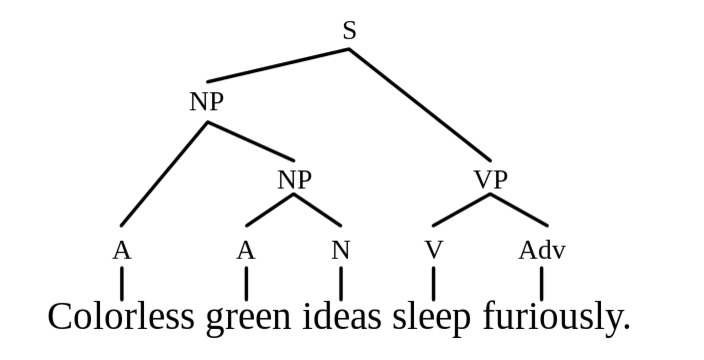
\includegraphics[width=0.9\linewidth]{nonsense.png}
	\caption {Constituency Parse Tree for 'Colorless green ideas sleep furiously'}
	\label{fig:nonsense}
\end{marginfigure}


\subsection{Constituency Parse Tree}
Interestingly, in natural language, the constituents are likely to be nested inside one another. Thus a natural representation of these phrases is a tree. Usually we use a consistency parse tree to display the parsing process. The constituency-based parse trees of constituency grammars distinguish between terminal and non-terminal nodes. Non-terminals in the tree are labeled as types of phrases (e.g. Noun Phrase), the terminals are the exact words in the sentence. Take 'John hits the ball' as an example, the syntactic structure of the English sentence is showed as below.

\begin{marginfigure}
	\centering
	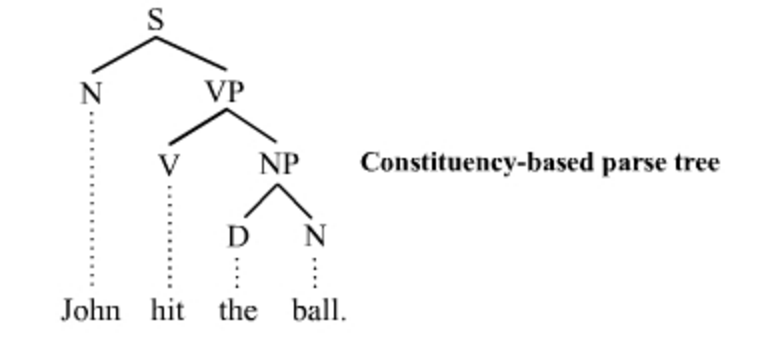
\includegraphics[width=0.9\linewidth]{ConstituencyParsing.png}
	\caption {Consistency Parse Tree for 'John hits the ball'}
	\label{fig:constParse}
\end{marginfigure}

We have a parse tree starting from root S, which represents the whole sentence, and ending in each leaf node, which represents each word in a sentence. We use the following abbreviation:

\begin{itemize}
\item S stands for sentence, the top-level structure.
\item NP stands for noun phrase including the subject of the sentence and the object of the sentence.
\item VP stands for verb phrase, which serves as the predicate.
\item V stands for verb.
\item D stands for determiner, such as the definite article "the"
\item N stands for noun
\end{itemize}


\subsection{Dependency-based Parsing}
Besides constituency parsing, there is another competing understanding of the logic of sentences, called 'dependency-based parsing'. The binary division of the sentence is rejected and replaced with the logic in terms of predicates and their arguments. It is a one-to-one correspondence compared to the one-to-one-or-more correspondence in constituency parsing. For every element in a sentence, there is just one node in the syntactic structure.

We parse the sentence 'John hits the ball' in terms of dependency-based parse tree. There is no distinction between terminal and non-terminal categories and it lacks the phrasal categories (S, VP, and NP) seen in the constituency-based counterpart above. It is simpler than the Constituent parse tree comparatively.

\begin{marginfigure}
	\centering
	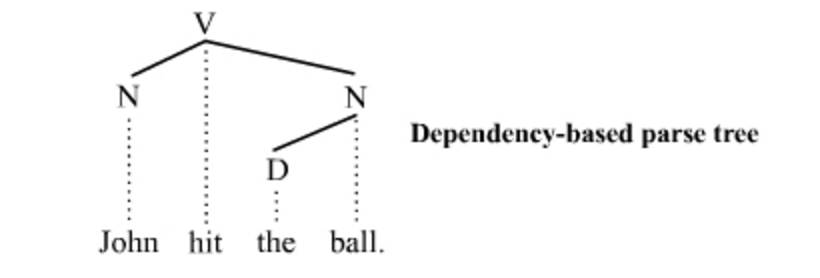
\includegraphics[width=0.9\linewidth]{denpendency.png}
	\caption {Dependency-based Parse Tree for 'John hits the ball'}
	\label{fig:dependency}
\end{marginfigure}

% \begin{marginfigure}%
%   \includegraphics[width=\linewidth]{img12}
%   \caption{Convolutional Neural Network}
%   \label{fig:img12}
% \end{marginfigure}


% \subsection{Defining Convolution}
% A bunch of inner products of a filter and a subset of a vector (or matrix) performed at the same time over strides of the full vector (or matrix).

% \begin{marginfigure}%
%   \includegraphics[width=\linewidth]{img13}
%   \caption{The Convolutional operation}
%   \label{fig:img13}
% \end{marginfigure}

% \subsection{Difference between Wide and Narrow Convolution}

% \begin{marginfigure}%
%   \includegraphics[width=\linewidth]{img14}
%   \caption{Wide and Narrow Convolution, or with and without zero-padding}
%   \label{fig:img14}
% \end{marginfigure}

% \subsection{Forming the input matrix}
% 1) one long vector
% Collobert and Weston (2011) Kim (2014)
% 2) a sentence matrix
% ()



% \subsection{Pooling and k-max Pooling}

% \begin{marginfigure}%
%   \includegraphics[width=\linewidth]{img15}
%   \caption{k-max pooling}
%   \label{fig:img15}
% \end{marginfigure}

% \subsection{Folding}


% \subsection{Dynamic Convolutional Neural Network}

% \begin{marginfigure}%
%   \includegraphics[width=\linewidth]{img16}
%   \caption{Dynamic Convolutional Neural Network}
%   \label{fig:img16}
% \end{marginfigure}

% Kalchbrenner actually dubs it a Dynamic Convolutional Neural Network for reasons we will explain soon.

% The model takes as input S, a “sentence image”, which is a (s x d)-matrix of word vectors that comprises a sentence’s words in the same order as they appear in the sentence. The model first zero pads the matrix on left and right to make S a (s+m-1 x d) matrix. Then performs a 1-dimension convolution (in the direction of the sentence progression) with S and a series of filters each of size m. Note m is usually between 3-10 depending on the developers preference. m=6 provided best results. The zero padding ensures that the width of the sentence matrix is never smaller than the size of the filters. This is called Wide-Convolution. It is important to note that the model utilizes f filters, f being some number of filters FOR EACH dimension in the word vector space. Making the matrix M that contains all the filters a  (f  x m x d) which is a 3rd-order tensor. And the output of the convolution step C a 3rd-order  tensor of size (s+m-1 x f x d). Kalchbrenner actually calls this matrix C, f separate feature maps, to align with what is discussed in Computer Vision as edge detectors. Note that no mixing of the dimensions has been performed. To fix this we fold over C by taking every other row and summing it with the previous one, shrinking our C by half (s+m-1 x f x d/2). Now for the “dynamic part”. We take the folded matrix and perform a dynamic k-max pooling step. K-max pooling is different than a normal max pooling step in that it returns the k max numbers rather than just the max. The dynamic piece comes into play in that we dynamically choose k depending on which layer we are in. The formula they use is arbitrary but gets smaller as we go deeper into the network. This is to ensure we do not lose information along the way, since we can have a sentence of arbitrary length.

% This whole process occurs one more time and then has a standard softmax output layer to deliver us a sentiment score. The DCNN results actually outperform RNTN in both the top level fine grained (5 label case) and the top level coarse accuracy (just positive or negative). However, the author does not include the results of the sub-phrase results. My assumption is that the RNTN performs better at small sentence/phrase lengths; otherwise Kalchbrenner would have included the results. Furthermore, it is intuitive that the DCNN performs more poorly on small phrases because the sentence matrix would consist of mostly the zero padding, giving much less information when convolved, and the information is essentially “watered down”.


\end{document}
